\acresetall

\chapter{Concept}\label{chapter:concept}
% This chapter introduces the architectural design of Component X. The component consists
% of subcomponent A, B and C.
% In the end of this chapter you should write a specification for your solution, including
% interfaces, protocols and parameters.
This chapter introduces the architectural design of plugin respect to the previously defined requirements.
Therefore the used development environment will be analyzed.
Followed by the initial architecture of the plugin to be developed.
Based on that the different layer of the system will be elaborated.

\section{Overview}
% The concept chapter provides a high-level explanation of your solution. Try to explain
% the overall structure with a picture. You can also use UML sequence diagrams for
% explanation.
% Figure 4.1 illustrates the situation between Alice and Bob. (sequence diagram from
% www.websequencediagrams.com)
\doit

% Docker Plugin as Vim Driver

\section{Development environment}
\doit

Open Baton is written in Java and is also partly ported to python and go.

\textbf{Python:}

\textbf{C/C++:}

\textbf{Node.js:}

\textbf{Go:}

\textbf{Java:}

Beside the fact that there is no complete implementation in the latter, the plugin will be written in Java.

The \ac{GUI} is a fundamental web client, which uses Angular.js as its main framework and some smaller tools like jQuery or the pretty famous bootstrap framework.

% Docker as container virtualization tool -> important: analysis for performance Docker vs. Hypervisor Virt.
% yaml for schema

% Open Baton has to be configured
% the plugins have to be installed (VIM Driver, VNFM(?))
% Docker has to be installed
% node must be able to execute docker and open baton client software

\section{Architecture of the system}
\doit

\begin{figure}[H]
    \centering
    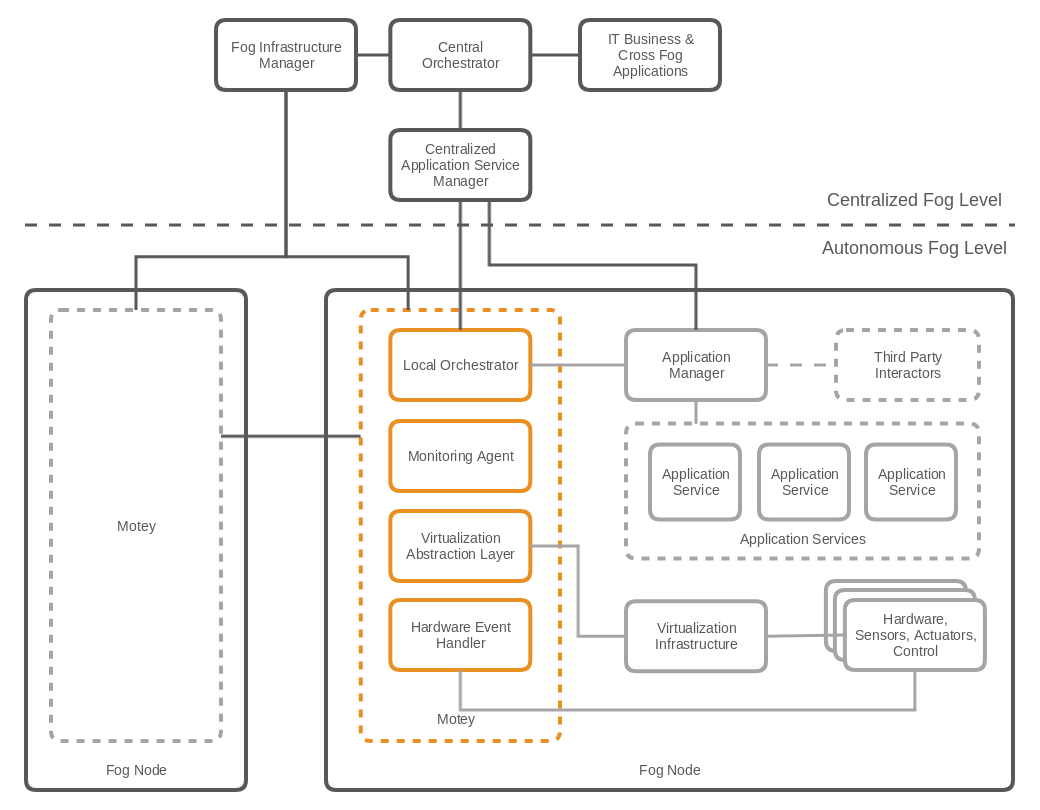
\includegraphics[width=\textwidth]{resources/images/initial_structure.png}
    \caption[Initial architecture design]{Initial architecture design}
    \label{fig:initial_architecture_design}
\end{figure}

% webserver, mqttserver, ZeroMQ endpoints und main logic aka core
% DI, RxPy,
% MVC ohne View -> keine spezielle architektur -> decoupled as much as possible -> DI hilft
% Sequenzdiagramm für Ablauf vom Deployment bis zum container: IMG_20170526_201659.jpg


\subsection{Data layer}
% daten lesen und schreiben
% tiny db -> easy to use, works well together with json in python
% sollte abstrahiert sein, damit es gut austauschbar ist -> Repository
% config.ini
\doit

\subsection{Orchestration layer}
% ist primär für das Blueprint handling zuständig
% -> bekommt daten via api und parst diese
% -> guckt ob lokal deployed werden kann oder externe Node benötigt wird
% sowie für die node-to-node Kommunikation
% -> Nodes registrieren sich beim starten der Engine
% -> können capabilities erfragen
% -> können container starten
% -> Sequenzdiagramme für die unterschiedlichen fälle erstellen
\doit

\subsection{Virtualization layer}
% val manager
% -> laden der plugins
% -> abstraction of plugin methods
% plugins
% -> abstract to to act as a interface
% -> concrete implementation of vals to implements specific virtualization tool
% -> yapsy as plugin tool
\doit

\subsection{Communication layer}
% API für externe tools
% MQTT für node discovery
% ZeroMQ für interne und externe Kommunikation mit einzelnen Komponenten und Tools
% -> beispiel labeling engine und node-to-node Kommunikation
\doit

\subsection{Capability Management}
% labeling engie für hardware events und andere third party apps
% plugins als capability
% werden in db gespeichert
% eine node kann andere nach capabilities fragen -> via ZeroMQ
\doit

\subsection{User interface}
\doit

\section{Conclusion}
\doit




% http://getcloudify.org/brochures/Heavy%20Reading%20NFV%20MANO%20Cloudify%20Snapshot.pdf
